\chapter[Yeniseian and Athapaskan Hydronyms]{\vspace{-25pt} Yeniseian and Athapaskan Hydronyms}

\sethandle{10125/24847}

\def\authorlast{Vajda}

% change author in three references below to the actual author name so that this name is unique and matches the \label commands just below and at the end of the chapter
\renewcommand{\beginchapter}{\pageref{vajda-ch-begin}}
\renewcommand{\finishchapter}{\pageref{vajda-ch-end}}
\label{vajda-ch-begin}



\thispagestyle{firststyle}


\chapauth{Edward Vajda}
\affiliation{Western Washington University}
\authortoc{Edward Vajda}

Jim Kari’s expertise in Athapaskan linguistics and life-long passion for cartography have yielded impressive advances in understanding the prehistory of Alaska and interior western Canada. His pioneering studies of Athapaskan hydronyms (Kari 1996, 2010) offer a potential model for investigating aboriginal place-naming systems in other regions of the world. The present article pays tribute to Jim’s work by applying his methodology to the study of Yeniseian substrate hydronyms in Siberia. Everything known about the river naming practices of the Ket and their extinct relatives——the Yugh, Kott, Assan, Arin and Pumpokol——is gathered together to explore the prehistoric dispersals of Yeniseian-speaking groups. A comparison is then made between Yeniseian and Athapaskan toponymic nomenclature and directional terms associated with riverine features of the traditional culture.



The article is organized as follows. Section~\ref{vajda:sec:1} discusses Athapaskan hydronyms in North America, mainly referencing work by Kari (1996, 2010). Section~\ref{vajda:sec:2} turns to Yeniseian hydronyms, relying upon the wealth of data published and analyzed by scholars from the former Soviet Union and the Russian Federation (Dul’zon 1959, Maloletko 2002, Werner 2002). Numerous Siberian river names found across a vast expanse of territory can be connected to documented Yeniseian languages through the phonology of their final combining forms (–\textit{ses},\textit{ }–\textit{čes},\textit{ }–\textit{sat},\textit{ }–\textit{šet},\textit{ }–\textit{tet}), which represent predictable reflexes of Proto-Yeniseian \textit{*s\=es} ‘river’. A separate subsection discusses river names ending in –\textit{tes or }–\textit{ši}, which may also reflect PY \textit{*s\=es} ‘river’, though left by otherwise undocumented Yeniseian languages. The discussion then turns to Yeniseian river names built using other morphological resources: -\textit{ul \~{} ur}, –\textit{lat}, –\textit{gat}, and –\textit{tɨm}. Section~\ref{vajda:sec:3} addresses the relevance of hydronyms to understanding Yeniseian prehistory. The probable location of the Proto-Yeniseian homeland is proposed on the basis of geographic and dialectal distribution of substrate river names. Section~\ref{vajda:sec:3} also cites findings from human genetics and comparative folklore studies that support a Yeniseian homeland in south-central Siberia or point to a connection with Na-Dene peoples. The semantics and morphology of Yeniseian and Athapaskan hydronyms as well as river-oriented directional terms are then compared. Directional verbs and adverbs belong to the core vocabulary of both families---a fact linked to the key importance of rivers and other bodies of water in the age-old seasonal lifestyle of boreal and sub-Arctic hunters-gatherers. The article’s conclusion draws together what can be deduced from hydronyms in light of earlier published evidence that Yeniseian and Na-Dene (Athapaskan, Eyak and Tlingit) are genealogically related---a proposal known as the Dene-Yeniseian connection (Vajda 2010). It might be apropos to mention at the outset that substrate hydronyms are not the best potential evidence of genealogical relationship between families, if only because of their propensity toward deformation through adoption by speakers of completely different languages, which tends to expose them to folk etymology.

\section{Athapaskan Hydronymic Districts in North America}\label{vajda:sec:1}

The existence of a robust and well-established Athapaskan morphological system for naming salient landmarks in the natural environment is evident virtually everywhere across interior northwestern Canada and Alaska. Kari (1996) mapped out seven distinct hydronymic districts within northern Athapaskan territory, each characterized by a primary final combining form (hydronymic formant) used to build names for flowing bodies of water. These districts appear to have remained stable over a considerable span of time (Kari 2010). The distribution of the seven primary hydronymic formants cuts across language boundaries, uniting individual Athapaskan language communities in ways not otherwise known to correspond to family-internal linguistic subgroupings: \textit{*–na’} (Denai’na, Ahtna, Lower Tanana, Kuskokwim, Deg Hitan, Koyukon), \textit{*–niq’ə} (Gwitchin, Middle Tanana, Upper Tanana, Tanacross, Han), \textit{*–nilənʲi} (Hare), \textit{*–deˑžʷə’} (Slave, Dogrib, Dene Sułine), \textit{*–tu’} (Northern Tuchone, Southern Tuchone, Tagish, Tahltan, Kaska), \textit{*–qʷəh} (Babine-Witsuwit’en, Dakelh, Chilcotin), and \textit{*–ɢah} (Tsesaut, Sekani, Beaver, Tsuut’ina). Figure~\ref{vajda-fig1}, reproduced from Kari (2010: 206), shows the distribution of these formants.



\begin{figure}
\centering
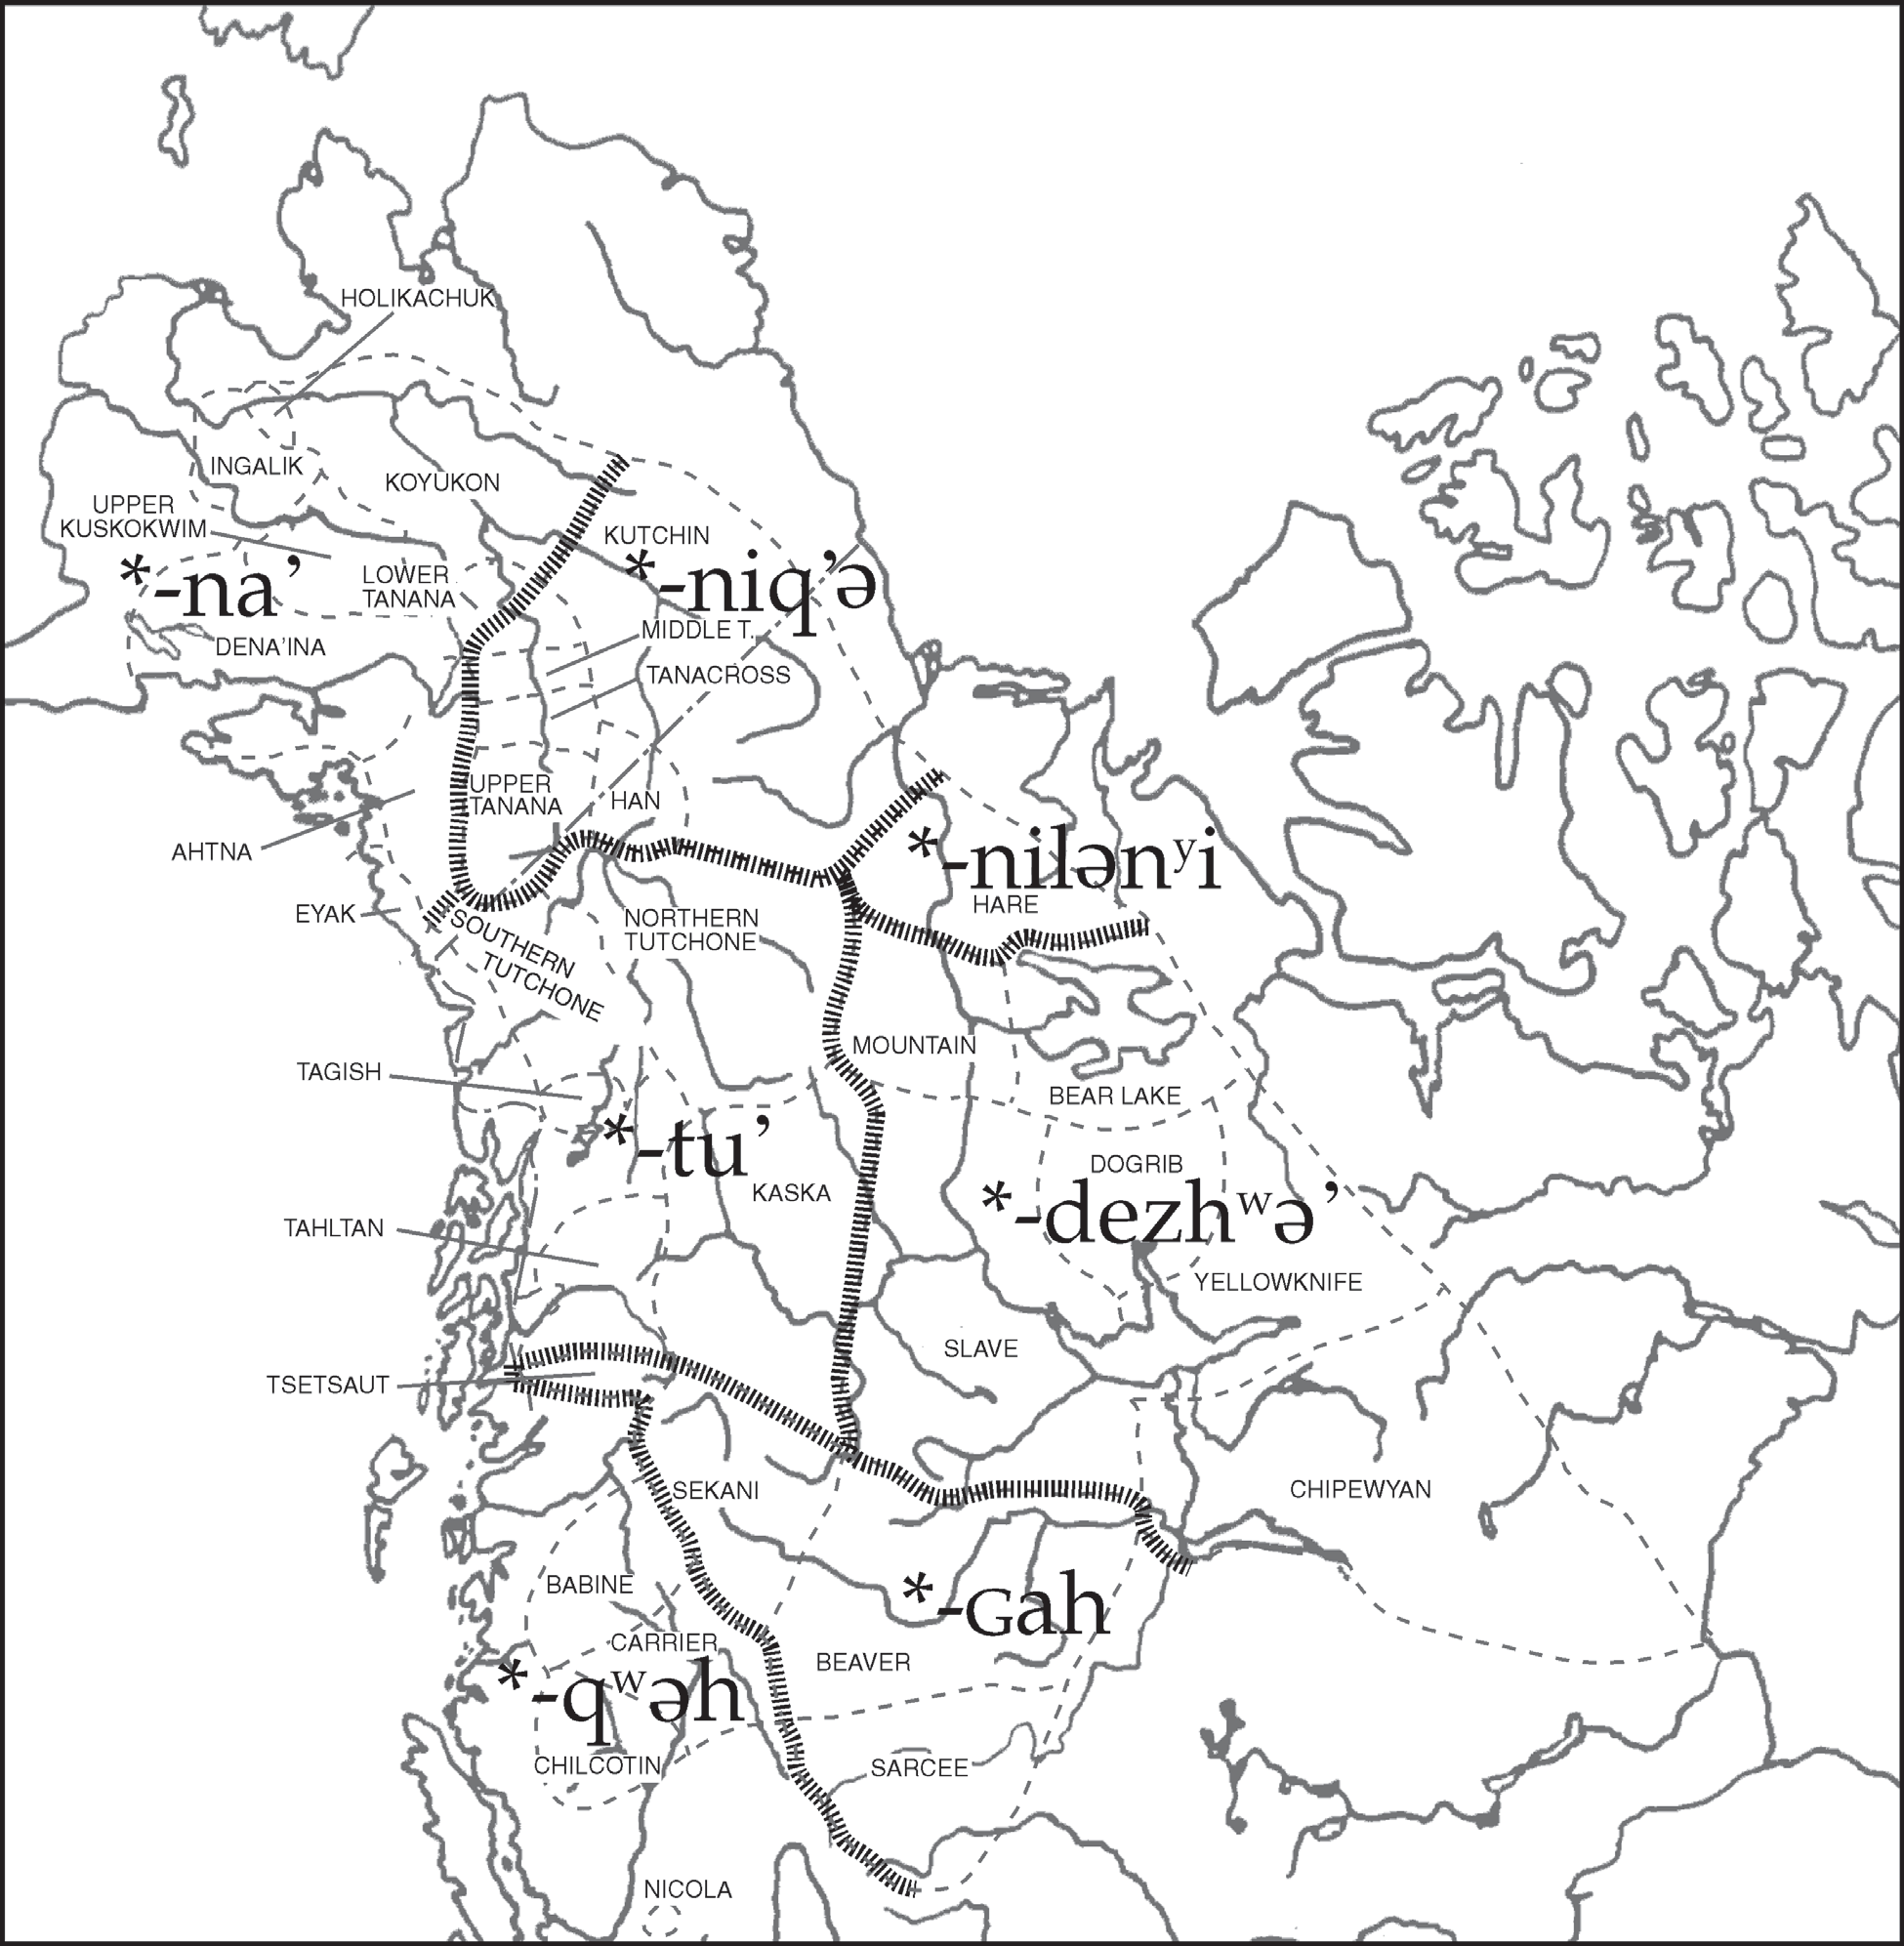
\includegraphics[width=0.7\textwidth]{figures/vajda-fig1}
\caption{Athapaskan hydronymic districts}\label{vajda-fig1}
\end{figure}


Only some of the river-name formants in Figure 1 have obvious etymologies (Kari 1996). Most of interior Alaska is divided into two hydronymic districts. The northeastern district is characterized by local reflexes of \textit{*–niq’ə}, which Kari etymologizes as meaning ‘upstream’. River names based on \textit{*–niq’ə} are in fact distributed upstream of river names belonging to the more western and southern Alaskan hydronymic district, characterized by the formant \textit{*–na}, a morpheme Kari relates to a verb root meaning ‘nomadize’. The etymologies of the two southernmost Canadian formants, \textit{*–qʷəh} and \textit{*–ɢah}, are not fully clear, though Kari (1996: 262) suggests they may have derived from morphemes meaning ‘along’ or ‘inside an enclosed space’. The formant \textit{*–nilənʲi} is unambiguously a nominalization of the verb root \textit{*lənʲ }‘current flows’; it also forms the only hydronymic district containing a single language (Hare). The formant \textit{*–deˑžʷə’}, found in river names across Arctic-draining areas of northwestern Canada, is the possessed form of Proto-Athapaskan \textit{*deˑšʷ} ‘sandbar, shoal, low island’. A cultural comparison with Yeniseian in Section 3 suggests a possible motivation for the semantic shift from ‘sandbar’ to ‘river’.

The western interior Canadian formant \textit{*–tu’} is the possessed form of the Proto-Athapaskan basic noun \textit{*tuˑ} ‘water’. Kari regards the area where the river-name formant \textit{*–tu’ }is prevalent as core Athapaskan territory, while formants used in other districts are likely to be later regional innovations (1996: 263-266). Harrington (1940) similarly viewed interior western Canada as some of the oldest territory occupied by Athapaskan speakers. Evidence for the primacy of \textit{*–tu’ }as a hydronymic formant comes from the fact that some river names in the other districts also have \textit{*–tu’}, whereas the remaining six formants are essentially limited to their respective districts as delimited in Figure 1.\textit{ }Kari (1996: 256) mentions the existence of four rivers in Ahtna territory with a final combining form \textit{*–tu’ }rather than \textit{*–na}, the typical formant for that area. The \textit{*–ɢah} district also contains river names in \textit{*–tu’}. Finally, in the Arctic-draining \textit{*–deˑžʷə’} district of northern Canada, \textit{*–tu’} ‘water’ regularly occurs as the final combining form in names of lakes rather than rivers (Kari 1996: 264).

Even if \textit{*–tu’} is indeed the original (or one of the original) Athapaskan hydronymic formants and the \textit{*–tu’} district is the nucleus from which the other districts later arose, the innovative formants \textit{*–na’}, \textit{*–niq’ə}, \textit{*–nilənʲi}, \textit{*–deˑžʷə’}, \textit{*–qʷəh}, and \textit{*–ɢah} still do not correlate with known sub-branches of the Athapaskan language family; it remains unclear how each became distributed across otherwise distinct linguistic boundaries. Concluding anything about the original Na-Dene hydronymic culture is made even more difficult by the fact that Tlingit and Eyak river-naming systems have not yet been systematically compared with Athapaskan. The Proto-Athapaskan nouns \textit{*deˑšʷ} ‘sandbar’ and \textit{*tuˑ} ‘water’ are cognate with the Eyak noun \textit{dehǯ }‘sandbar’ and Eyak preverb \textit{tu\textsuperscript{ʔ}}\textit{ }‘water’. The Tlingit nouns \textit{xág}\textit{\textsuperscript{w}} ‘sandbar’ and\textit{ héen} ‘water’ are used in complex Tlingit hydronyms (Thornton 2008: 56) but they do not appear to be cognate with any of the Athapaskan hydronymic formants discussed in Kari (1996). Because no shared system of toponymic morphology has yet been reconstructed even to the level of Na-Dene, any deeper comparison with Yeniseian river names must be limited, at least for the present, to identifying structural or semantic parallels rather than undertaking a genealogical comparison. Still, as will be argued below, a comparison of Dene-Yeniseian hydronymic nomenclature is illuminating for a number of reasons.

%section 2
\section{Yeniseian Substrate Hydronyms in Siberia}\label{vajda:sec:2}


The situation with respect to pre-Russian hydronyms in central Siberia differs from the traditional Athapaskan areas of North America is three salient respects. First, as already noted, Athapaskan hydronyms form ‘districts’ that cut across language boundaries, whereas the most common Yeniseian river-name formants display phonological traits connecting them to particular languages or branches of the family. Because Yeniseian hydronymic formants parallel established family-internal sub-divisions---and this is particularly true of river names built with final combining forms derived from Proto-Yeniseian \textit{*s\=es} ‘river’---they are of great value in tracing the prehistoric location of groups speaking particular Yeniseian daughter languages. Because the distribution of Athapaskan hydronymic formants do not match other known facts about the family’s historical diversification, they are not so readily helpful for tracing prehistoric population movements.

Second, the vast majority of recorded Yeniseian toponyms are specifically river names (potamonyms). Native Yeniseian names of lakes, hills, rocky outcrops, forest uplands, etc., survive only rarely in substrate areas; such toponyms were mostly recorded in territory still occupied by Yeniseian speakers when Russians initiated the first European contact after 1600. A logical reason for the overwhelming survival rate of substrate river names as opposed to other Yeniseian toponyms is proposed in Section 3 below. Most Yeniseian river names form substrate complexes that survive only through the medium of a second (if not a third) linguistic layer, and only a few were recorded directly from intact Yeniseian-speaking communities. By contrast, Athapaskan landscapes abound in toponyms naming the full gamut of natural geographic features. The fact that Athapaskan hydronyms were recorded by Jim Kari and other linguists directly from fluent native speakers, not merely by analyzing substrate relics left by long vanished populations, further contributes to the richness of the North American corpus in contrast to the much thinner record of Yeniseian toponyms in Siberia.

Finally, Athapaskan territory is saturated with native place names to the remarkable exclusion of any other layer of pre-European toponyms. This indicates either the family’s great age in the given territories, as argued in Kari (1996, 2010), or a strong cultural propensity to replace non-native place names in any newly acquired territory. The latter possibility is suggested by the fact that Navajo and Apache areas of the American Southwest, Athapaskan place names likewise blanket the landscape despite the known shallow time depth of occupation by Athapaskan speakers. to provide further insight into the link between toponymy and Athapaskan expansions, the Pacific Coast Athapaskan and Apachean areas should be compared with Northern Athapaskan. Whether due to time depth of occupation or cultural naming practices, or to both factors, Northern Athapaskan territory shows little or no sign of earlier linguistic substrates. Yeniseian-speaking peoples, on the other hand, were definitely only one ethnic component from among several known indigenous language families that contributed to the pre-Russian toponyms that survive today in south-central Siberia. Yeniseian substrate hydronyms are of great value in understanding ethnic and linguistic population replacements throughout south-central Siberia, a fact convincingly established by the great Siberian scholar Andreas P. Dulson (Dul’zon 1959). Most of the pioneering scholarship on Yeniseian toponyms by Dulson and other soviet era scholars appeared in local Siberian publications that are difficult to access. All of these important works, which number in the dozens, are listed in Vajda (2001: 372), where each is provided with a detailed English annotation.

The discussion below elaborates on the significance of these points of contrast between Yeniseian and Athapaskan river names: 1) the degree to which hydronymic formants match other known aspects of family-internal diversification, 2) the richness or poverty of the recorded toponymy, and 3) whether or not river names are interspersed with those of other language families.

\subsection{Hydronyms from Proto-Yeniseian \textit{*s\=es} ‘River’}

The Kets today live along the middle reaches of the Yenisei from the Mountain Tunguska north to the Kureika river, just above the Arctic Circle. As a nationality in the Russian Federation, they number 1209 people according to the 2010 census, although only a few dozen elderly people are fluent in any the three surviving dialects of the traditional language (Northern Ket, Central Ket, Southern Ket). When Russian fur traders and Cossack adventurers penetrated the Yenisei watershed in the decades following Yermak’s attack on the Khanate of Kuchum in 1582, the Ket hunting bands were only one of several linguistically distinct Yeniseian populations they encountered. Figure 2, redrawn from Vajda (2001: xxvii), shows the approximate distribution of Yeniseian-speaking groups as recorded in the 17\textsuperscript{th} century by Russian fur tax (\textit{yasak}) collectors. For more historiographic detail on Yeniseians in the first century after the Russians’ arrival, see Dolgikh (1960: 143-150, 184-191, 204-206, 222-275, and especially the back-cover foldout map insert). Present-day locations of Ket populations are marked in Figure 2 with stars.

\begin{figure}
\centering
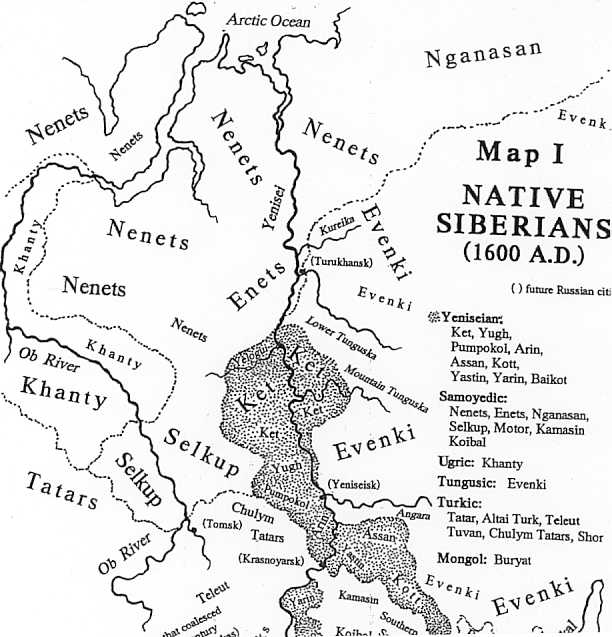
\includegraphics[width=0.7\textwidth]{figures/vajda-fig2}
\caption{Documented Yeniseian territories in 1600}
\label{vajda-fig2}
\end{figure}


Each language area shaded in gray contains river names with a formant reflecting Proto-Yeniseian \textit{*s\=es} ‘river’: Ket, –\textit{ses}, Yugh –\textit{čes},\textit{ }Arin –\textit{set}, Kott–\textit{šet }and Pumpokol\textit{ }–\textit{tet} (Werner 2005: 316-318). These variants show the regular reflexes of Proto-Yeniseian \textit{*s}, which yielded /t/ in Pumpokol and the sibilant /š/ in Kott (and in the closely related Assan). The final /t/ in Arin \textit{set} and Kott\textit{ šet }appears to have resulted from dissimilation of coda /s/ following an onset sibilant or shibilant. This type of dissimilation in Kott and Arin (but not Ket) is evident in at least one other item of basic vocabulary: Ket \textit{se’s} ‘larch (tree)’, but Arin \textit{čit} ‘larch’ and Kott-Assan \textit{šet} ‘larch’ (Werner 2005: 306). As for Yugh hydronyms, although the Ket and Yugh word for ‘river’ is \textit{s\=es}, the Yugh combining form is normally \textit{–čes}, in contrast to Southern and Northern Ket \textit{–ses} and Central Ket \textit{–šeš.} The change of syllable anlaut /s/ to /č/ in the middle of compounds also occurs sporadically in Northern Ket (cf. Southern Ket \textit{bənsaŋ} ‘it is not’, but Northern Ket \textit{bənčaŋ} \~{} \textit{bənsaŋ}).

Yeniseian-derived river names that survive as substrate toponyms among the current Russian- or Turkic-speaking populations of southern or western Siberia are built using virtually identical final combining forms that can easily be connected to a particular Yeniseian daughter language: \textit{–ses \~{} sis \~{} zis \~{} sas \~{} zes \~{} zas }(Ket), \textit{–čes }(Yugh), \textit{–set \~{} sat \~{} zet \~{} zat}, also\textit{ –kul }(Arin), \textit{–šet \~{} čet }(Kott), \textit{–ul }(Assan), \textit{–tet \~{} tat \~{} det \~{} dat }(Pumpokol). Variants such as \textit{zis \~{} sas} arose through accommodation to Turkic or other languages spoken by pastoral peoples who took over these areas. Alternation between /e/ and /a/ reflect the pattern of front/back vowel harmony typically found in the pronunciation of Turkic and most other Inner Eurasian languages, but lacking in the Yeniseian languages themselves.

Substrate river names with a final-combining form derived from PY \textit{*s\=es} ‘river’ are also distributed far beyond the areas documented by Russians as being inhabited by Yeniseian-speaking hunter-gatherers. Yeniseian river names are thus uniquely useful for tracing the former distribution and expansion of individual Yeniseian daughter languages. It is possible to postulate four distinct Yeniseian substrate zones based on known family-internal sub-divisions, as in \REF{vajda-substrate}.

%Table 1: Yeniseian substrate hydronymic zones based on reflexes of \textit{*s\=es} ‘river’

\begin{exe}\label{vajda-substrate}
\ex Yeniseian substrate hydronymic zones based on reflexes of \textit{*s\=es} ‘river’
\begin{xlist}
\ex Ketic \textit{*–ses} ({\textgreater}\textit{ ses \~{} šeš \~{} sis \~{} zis \~{} sas \~{} zes \~{} zas \~{} čes}) representing the known Ket dialects, as well as Yugh (\textit{čes}), and probably other closely related but otherwise undocumented language forms;
\ex Arinic \textit{*–set} ({\textgreater} \textit{set \~{} sat \~{} zet \~{} zat}) representing the documented Arin language and possibly other closely related but undocumented language forms;
\ex Kottic \textit{*–šet }({\textgreater} \textit{šet \~{} čet}) representing the documented Kott dialects, as well as Assan, though documented Assan potamonyms normally end in \textit{–ul} rather than a reflex of \textit{*–šet}), and possibly other closely related but undocumented language forms;
\ex Pumpokolic \textit{*–tet }({\textgreater} \textit{tet \~{} tat \~{} det \~{} dat}) representing the documented Pumpokol language and possibly other closely related but undocumented language forms.
\end{xlist}
\end{exe}

Figure~\ref{vajda-fig3} shows the location of \textit{*s\=es}{}-derived substrate hydronyms beyond the areas where 17\textsuperscript{th} century Russian fur tax collectors actually encountered Yeniseian-speaking groups (marked in gray, as in Figure 2). The placement of substrate hydronymic labels is unavoidably impressionistic. For example, if a 300-kilometer river carries a substrate Yeniseian name, it is not possible to know whether the original speakers nomadized along the river’s entire length or only near one location. Compact geographic clusters of a particular hydronymic formant, however, strongly indicate that speakers of a particular Yeniseian language variety once occupied the general area. Four hydronymic notations correlate with the four main documented Yeniseian daughter branches: Ketic (Ket-Yugh) \textit{ses}, Arinic \textit{set}, Kottic (Kott-Assan) \textit{šet}, and Pumpokolic \textit{tet. }Secondary phonetic variation (\textit{–zas, –sas}, \textit{–sis}, etc.), presumably caused by minor dialectal variation or adaptation into a superstrate language is ignored. The circled area is identified as the probable Proto-Yeniseian homeland, a proposal to be discussed in Section~\ref{vajda:sec:3}.


\begin{figure}
\centering
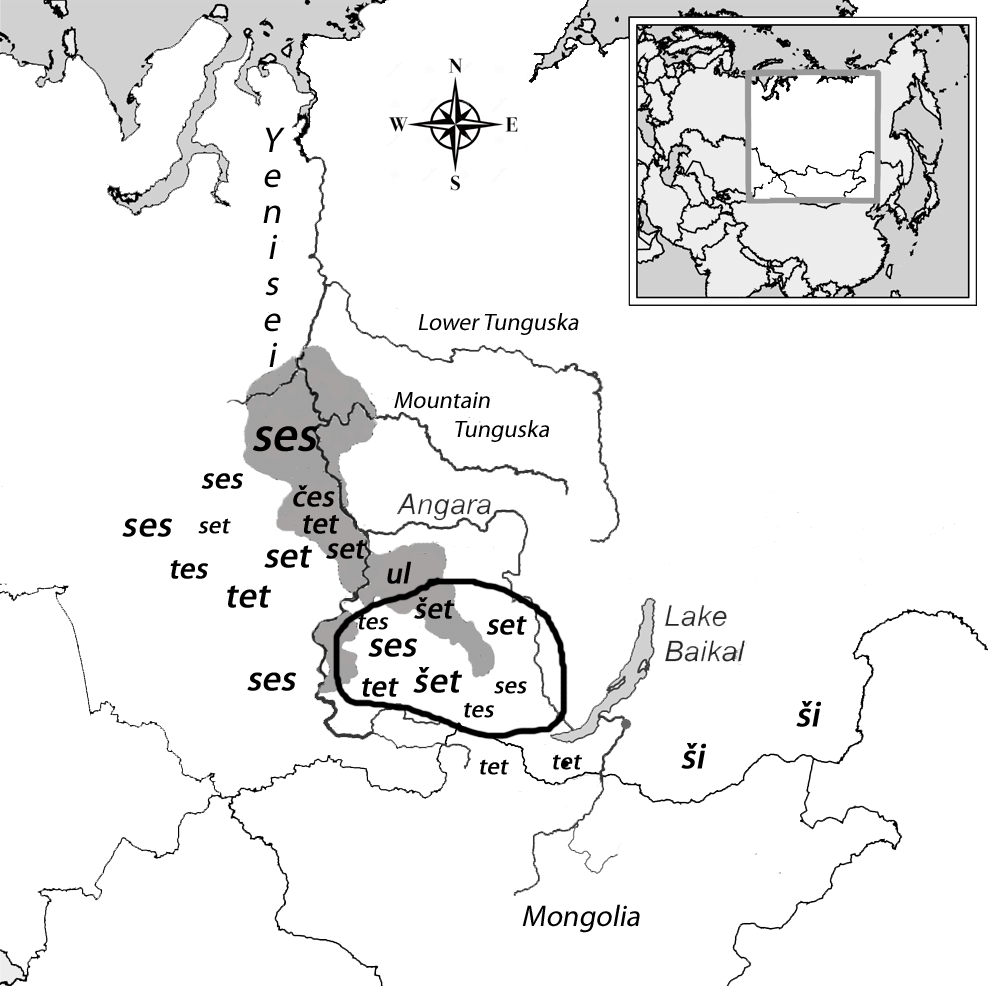
\includegraphics[width=0.7\textwidth]{figures/vajda-fig3}
\caption{Former distribution of Yeniseian languages shown by substrate toponyms}\label{vajda-fig3}
\end{figure}

%Figure 3: Former distribution of Yeniseian languages shown by substrate toponyms.



Two of the hydronymic notations in Figure~\ref{vajda-fig3}---\textit{tes} and \textit{ši}---do not correlate with any known Yeniseian language. They also plausibly derive from Proto-Yeniseian \textit{*s\=es} ‘river’ and may represent vestiges of extinct Yeniseian languages not otherwise documented. River names with the final combining form \textit{–tes \~{} tas \~{} tɨš} \textit{\~{} des \~{} das }appear in large areas of south and western Siberia. If these river names do reflect evolution from PY \textit{*s\=es} ‘river’, as originally proposed by Dul’zon (1959), then the initial plosive /t \~{} d/ could conceivably have arisen in any of several ways. Such a Yeniseian daughter language may have undergone a secondary dissimilation of anlaut /s/ to /t/ in syllables ending in a sibilant (\textit{*s\=es} {\textgreater} \textit{tes}). In that case, the \textit{*–tes }river names would probably form an extension of the Ketic zone. Or, alternatively, the final combining forms \textit{–tes \~{} tas \~{} des \~{} das} might preserve the Yeniseian 3\textsuperscript{rd} person possessive connector prefix \textit{d}{}- (\textit{*d-s\=es} {\textgreater} \textit{tes}), though this morphological trait is not observed in river names associated with known Yeniseian languages. The most intriguing possibility is that the original Proto-Yeniseian form of ‘river’ may have been \textit{*tes} or \textit{*des} rather than \textit{*s\=es}, with initial /s/ in all documented languages arising from long distance sibilant assimilation (\textit{*tes }or\textit{ *des} {\textgreater} \textit{ses},\textit{ set}, etc.). This would make the earliest Yeniseian word for ‘river’ resemble Proto-Athapaskan \textit{*deˑšʷ} and Eyak \textit{dehǯ}. However, the possibility that long distance anlaut sibilant assimilation yielded \textit{*s\=es} from earlier \textit{*d\=es} in the language ancestral to Ket appears to be contradicted by the fact that no such assimilation occurred in phonologically similar words (cf. Southern Ket \textit{d\=es} ‘eye’, \textit{tòs} ‘raising’, \textit{do’s} ‘anthropomorphic spirit image fashioned from a log’, etc.). Most \textit{*–tes }river names are found in southern or western Siberia, though one is located in northern Ket territory: the Luntes tributary of the Kureika river. “Luntes” appears to derive from \textit{l\=un} ‘grayling (fish)’ + \textit{s\=es} ‘river’ via deaffrication of original \textit{lun-čes}. It is not connected with the more numerous south and west Siberian river names of undetermined linguistic provenance (Kajtes, Baktas, Kɨtas, Utaz, etc.), though it is possible that the final combining form in these names too could have arisen through secondary affrication and deaffrication in whatever Yeniseian language or dialect they derive from. The example provided by the river name “Lunches” demonstrates how the presence of a single substrate toponym can generate ambiguous conclusions. Areas with multiple examples of the same morphological type of substrate toponym are more useful in exploring linguistic prehistory. Dulson’s identification of a Yeniseian origin (Dul’zon 1959) for river names in \textit{–tes \~{} tas \~{} tɨš} \textit{\~{} des \~{} das }in southern and western Siberia (conceivably including the name of the large Irtysh river), remains the most plausible interpretation. These toponyms form compact zones and the initial combining forms in some of them appear to have Yeniseian etymologies (Maloletko 2002: 152-154; Werner 2002, vol. 3: 68-69). These two facts make it unlikely that all southern and western Siberian \textit{–tes }river names arose through random secondary affrication followed by deaffrication, as occurred in the solitary case of Northern Ket “Luntes”.

River names ending in \textit{–ši \~{} či} found in southeastern Siberia may also reflect PY \textit{*s\=es} ‘river’, though in no recorded Yeniseian language does the final consonant of this formant elide. Many \textit{–ši }river names are found across Zabaikalye, well to the east of Lake Baikal and extending as far as Heilongjiang (formerly Manchuria) and the Amur basin (Zhamsaranova 2015); they appear to be widely distributed in these territories, which were occupied by Buryat Mongols or Ewenki (Tungusic) pastoralists when Russians penetrated the area. The possibility of Yeniseian river names in eastern Siberia, closer to the Pacific, is intriguing for understanding the geography of the Dene-Yeniseian connection, but more work needs to be done to strengthen the case that toponyms in \textit{–ši} are, in fact, of Yeniseian linguistic origin.

\subsection{Yeniseian River Names Without \textit{*s\=es}}

Interspersed across areas containing Yeniseian hydronyms built with \textit{*s\=es} ‘river’ are other Yeniseian river names built using completely different formants. Chief among these are river names containing reflexes of Proto-Yeniseian \textit{*x\=ul} ‘water’. These are particularly prevalent in the Assan areas (Werner 2002 vol. 3: 61-64), where the final combining form \textit{–ul} (less often rhotacized to \textit{–ur}) appears more frequently than Kottic \textit{–šet}. This pattern correlates with 18\textsuperscript{th} century word lists, where the free form \textit{ul} (rather than \textit{šet}) is recorded as meaning both ‘river’ and ‘water’ in Assan (Werner 2005: 144). The final combining form \textit{–kul} in river names correlates with Arin, and also matches the Arin free noun \textit{kul} ‘water’. Arin river names in \textit{–kul} tend to occur in the same general areas as Arin river names in \textit{–sat}. The reason behind the difference in morphological formant is unclear. Yugh \textit{\=ur} ‘water’ also shows up occasionally in Yugh territory river names as the final combining form \textit{–ur}. River names ending in \textit{–ur }are also found in south Siberia east of Lake Baikal (Zhamsaranova 2015), including the same areas containing the possibly Yeniseian-derived river names in \textit{–ši}. Hydronyms ending is a syllable with the shape \textit{–ur} are also well represented in the Amur watershed stretching eastward to the Pacific, and include the name ‘Amur’ itself, though there is no evidence that any of them are connected with Yeniseian \textit{*x\=ul} ‘water’. It is difficult to etymologize the internal structure of east Siberian \textit{–ur} hydronyms or identify any of them as Yeniseian in the absence of additional evidence showing that Yeniseian-speakers lived that far east of Lake Baikal. Yeniseian hydronyms that are fully etymologizable most often name some economically salient feature of the riverine environment, such as the type of fish, plant or animal found there and transparently conform to the structure: modifier noun (or adjective) + head noun. The initial portions of the various eastern Siberian –\textit{ur} river names cannot at present clearly be identified with specific Yeniseian words.

Many areas of south and west Siberia that contain river names with unambiguous reflexes of PY \textit{*s\=es} ‘river’ or \textit{*x\=ul} ‘water’ also contain river names ending in \textit{–kat }(or its substrate phonetic variants \textit{–ket} \~{} \textit{gat} \~{} \textit{get}) or \textit{–lat }(or \textit{–let}). Werner (2012) has argued persuasively that \textit{–kat \~{} ket }originated from a Proto-Yeniseian root meaning ‘clan’ (cf. Modern Ket \textit{kə’t} ‘children of the same mother’ and Kott \textit{kat} ‘children’). This also explains why \textit{–kat }\~{} \textit{ket} \~{} \textit{gat} \~{} \textit{get} river names are found primarily in areas alongside either Ketic \textit{–ses} or Kottic \textit{–šet}. Presumably, such names derived from ethnonyms of Yeniseian-speaking kin groups who nomadized near the given river and who met and traded there with other nationalities, thus transferring their clan designation to an alien linguistic community as the name of the given river.

This analysis can further be extended to river names with the formant \textit{–lat }\~{} \textit{let}. These appear to have the same etymology, but reflect Arin and Pumpokol phonology: cf. Arin \textit{alpolat} ‘child’ and Pumpokol \textit{hiluŋla} ‘child’, where the final syllables \textit{{}-lat} and \textit{{}-la} are cognate with Ket \textit{kə’t} ‘children of the same mother’ and Kott \textit{kat} ‘children’. The odd sound correspondence Ket /k/, Kott /k/, Arin /l/, Pumpolkol /l/ occurs in other words, as well, such as the noun ‘winter’: Arin \textit{lot}, Pumpokol \textit{lete}, Kott \textit{kêti}, Southern Ket \textit{kət}.

Other river names derive from words having to do with nomadizing. \ The geography of the seasonal nomadic cycle is similarly reflected in Ket river names ending in \textit{–kaŋ}, which are derived transparently from the Southern Ket noun \textit{kàŋ }‘winter hunting trail’. These tend to be small, upland tributaries, especially those in the Mountain Tunguska watershed, along which Kets traveled during their winter hunting forays, whereas \textit{–ses} names larger rivers where Ket families camped during the warm season; see Werner (2002, vol. 3: 34-42) for a list of \textit{–kaŋ} tributaries interspersed with \textit{–ses} river names. The use Southern Ket \textit{kàŋ }‘winter hunting trail’, a morpheme associated with nomadizing, as a river name formant finds a semantic parallel in the Alaskan Athapaskan hydronym formant \textit{*–na}, if the latter is indeed connected with verb forms meaning travel in a group.

Areas with river names in Ketic \textit{–ses }or\textit{ –kat}; Kottic \textit{–set}, \textit{–kat }or\textit{ –ul}; Arinic \textit{–set}, \textit{–kul }or\textit{–lat}; and Pumpokolic \textit{–tet} or\textit{ –lat} also contain a scattering of river names built with the element \textit{–tɨm \~{} tom}. The tom river, on which the eponymous city of tomsk is located, also belongs in this group. The tomsk area falls inside the Pumpokolic substrate zone, and in fact the word \textit{tom} in 18\textsuperscript{th} century Pumpokol word lists is glossed as ‘river’. Although the basic Proto-Yeniseian noun for ‘water’ is \textit{*x\=ul}, with reflexes in every daughter language, there is some evidence that a root with a form something like \textit{*to \~{} tu \~{} tom }also meant ‘water’ in Yeniseian. In addition to substrate river names in \textit{–tɨm \~{} tom} found in areas representing all of the documented Yeniseian daughter branches, Ket and Yugh have a number of complex word containing this morpheme in the meaning ‘water’. These include: Ket \textit{t\={o}ˑgde} ‘river bend’, ‘small bay in river’ {\textless}\textit{ to }‘water’ + \textit{ged }‘bend’; Ket \textit{tɨmoks}\textbf{\textit{ }}‘wood shavings used for cleaning of dishes {\textless}\textbf{\textit{ }}\textit{tɨm }‘water’ + \textit{\={o}ˑks }‘wood’; Ket \textit{toʁ\'{o}jiŋ}, Yugh \textit{toχojiŋ }‘drying’ {\textless} \textit{to }‘water’ + \textit{qoj }‘dry’ + \textit{ŋ }(action nominal suffix); Ket \textit{totaləŋ}, Yugh \textit{totarɨŋ }‘shallow’ {\textless} \textit{to} ‘water’ + \textit{tol} ‘low’ + \textit{ŋ} (adjective suffix); Central Ket dialectal \textit{tɨmet} ‘lake’ {\textless} \textit{tɨm} ‘water’ + \textit{et }‘surface (?)’; and Central Ket dialectal \textit{tamtul} ‘lake’ {\textless} \textit{tɨm} ‘water’ + \textit{tul} ‘cavity, bottom, low area’. The alternation between nasal and non-nasal codas in \textit{to \~{} tu \~{} tom \~{} tɨm }is unexplained and complicates the obvious suggestion of cognacy with Proto-Athapaskan \textit{*tuˑ} ‘water’, which shows no nasal coda in any modern Athapaskan dialect (Vajda 2010: 81). Also complicating the Dene-Yeniseian comparison is the fact that the most prevalent Yeniseian word for water is clearly \textit{*x\=ul}, which does not seem to have a cognate in any Na-Dene language.

The largest rivers in the Ket areas, which represent the most northern portions of Siberia known to have ever had Yeniseian-speaking inhabitants, are not built with any of the formants typically found in Yeniseian names for smaller tributaries (\textit{–ses}, \textit{–tɨm}, \textit{–ul}). The Yenisei river itself is called \textit{q\=uk}, a name with no clear etymology; see Janhunen (2009: 73-74) for a cogent discussion of the origins of various ethnic designations for the Yenisei river. The term is more likely to be a substrate hydronym of unknown origin than the result of polysemy from the homonymous Ket noun \textit{q\=uk} ‘hole, perforation’. Ket folk etymology associated the native name for the Yenisei with the hole that the great shaman Doh created in a rock cliff. This allowed the Yenisei to flow northward, giving the Ket people a route of escape from the malevolent female deity Hosedam. The Kets also refer to the Yenisei using the descriptor \textit{\=uls }‘wide expanse of water’ ({\textless} Pre-Ketic \textit{*\=ul} ‘water’ + \textit{*wes} ‘open space’), but this is not a proper noun uniquely applied to the Yenisei, as it can be applied to any broad expanse of water.

The large eastern tributaries of the Yenisei, which flow down from the Central Siberian Plateau, have names mainly built with \textit{qol \~{} qo’l}. These include \textit{Qo’l} or \textit{Qaʁol }‘Mountain (or Stony) Tunguska’ ({\textless} \textit{qà }‘big’ + \textit{qo’l}), as well as \textit{Baŋnoqol} ‘Lower Tunguska’, \textit{Boɣenol} ‘Dry Tunguska’. The latter two names may have the initial combining form \textit{ba’ŋ }‘earth’, referring to rapids and swiftly moving water; cf. Ket \textit{bannej} ‘splashing of water against objects’, \textit{baŋes \~{} baŋnas }‘rapids’ {\textless} \textit{*ba’ŋ} ‘earth’ + \textit{*wes} ‘open space’. These are turbulent rivers that descend at a steeper gradient than the low-lying western tributaries of the Yenisei. Therefore, the formant \textit{qol} is unlikely to have derived polysemously from Ket \textit{qo’l }‘calm water, small bay’ ({\textless} \textit{*q\={u}g}\textbf{\textit{ }}‘calm’ + *\textit{\={u}l} ‘water’). Also unexplained are the Yeniseian names for the Bakhta river: Ket \textit{Baqtoq}, Yugh \textit{Beaχtaχ}, which are unlikely on phonological grounds to contain \textit{*to} ‘water’ as their final combining form. More likely, the shape of these names represent a form originally ending in the syllable \textit{–qol}, which has reduced to coda /q/. This is unproven but would be in keeping with the fact that the Bakhta is also an eastern tributary of the Yenisei, draining from the same Central Siberian Plateau as other river names with the final combining form \textit{–qol}.

Finally, a number of river names, mostly in Yugh territory, are built with the syllable \textit{sɨm}. These include the Sym river itself and some of its tributaries (Werner 2002, vol. 3: 42-44). River names with final combining form –\textit{sɨm} reflect a pre-Yeniseian substrate of unknown origin, since the anlaut /t/ in the Yeniseian formant\textit{ –tɨm} would not have become /s/ in Ket or Yugh. Alekseenko (1975) suggested that river names with \textit{sɨm} were left by the original Yugh tribe, who did not speak a Yeniseian language and whose ethnic designation was transferred to the Ketic-speaking bands who later moved into this area and became known as the “Yugh” or “Sym-Ket”. The prevalence of major non-Yeniseian hydronyms in the lands that Ket and Yugh people actually inhabited during the historic period can be explained by the relatively recent migration of Ket and Yugh family groups from more southerly areas. These migrations are well attested in Ket folklore (Alekseenko 1967), early Russian fur tax records (Dolgikh 1960), as well as on modern maps by the presence of many \textit{–ses} river names in areas far to south or west of today’s Ket villages located in the north of the modern Turukhansk District in Krasnoyarsk Krai (Dul’zon 1959).


\section{Hydronyms and the Dene-Yeniseian Connection}\label{vajda:sec:3}

Before turning to a morphological comparison of Yeniseian and Athapaskan river names, it would be useful to mention the existence of a small number of Yeniseian toponyms naming other geographic objects and consider why the names of small to medium-sized rivers are so overwhelmingly prevalent in Yeniseian substrates in contrast to other toponyms.

Lake names in Ket-Yugh areas often end in the formant \textit{–de}, derived transparently from the Ket and Yugh noun \textit{de’} ‘lake’: Ket \textit{Dɨnde} {\textless} \textit{dɨn} ‘spruce’ + \textit{de’} ‘lake’, \textit{tomulde} {\textless} \textit{t\=um} ‘dark’ + \textit{\=ul} ‘water’ + \textit{de’} ‘lake’. The names of small streams in the Ket areas (in contrast to rivers) sometimes contain the final combining form \textit{–qoks}, from the noun \textit{qoks} ‘stream, brook’, less often \textit{–doks}. The final \textit{{}-s} in\textit{–qoks} and \textit{–doks} resembles the nominalizing suffix \textit{*-si}, which would suggest that \textit{*qok} and \textit{*dok} were verbal roots (cf. the Ket verb base\textit{ -doq} ‘jump, spring, fly’). Wooded uplands often carry names ending in \textit{–lɨt}, from \textit{lɨ’t }‘forest, forested upland’, such as \textit{qonlɨt} {\textless} \textit{qo’n} ‘fir, conifer’ + \textit{lɨ’t }‘upland’, \textit{qoqŋlɨt} {\textless} \textit{qokŋ} ‘pine forest’ + \textit{lɨ’t }‘upland’. While there are no true mountains in the northern Ket areas, the Shor district just north of the Altai preserves a few substrate oronyms (mountain names) with the final combining form –\textit{sai}, probably correlating with Kott dialectal \textit{džii} \~{} \textit{gijlin} ‘mountain(s)’ (Werner 2005: 310). These forms reflect Pre-Kottic *\textit{ǯi:l} (plural\textit{ *ǯi:l-in}), a probable cognate of Proto-Athapaskan \textit{*ʒəł} ‘mountain’ and Tlingit \textit{gudl} ‘mound, hump’. Athapaskan uses reflexes of \textit{*}–\textit{ʒəł} in naming mountains above the timberline. It is possible that Pre-Ketic \textit{*lɨ’d}\textit{\textsuperscript{j}} ‘upland’ is a metathesized form of earlier \textit{*d}\textit{\textsuperscript{j}}\textit{ɨl} ‘mountain’, given the prevalence of innovative metathesis in Ket-Yugh and its relative absence in Kott-Assan. The Ket formants \textit{–qoks} and \textit{–doks }are not obviously cognate with Na-Dene toponymic elements.

Except for river names, very few Yeniseian toponyms survive in substrate areas. Outside the modern Ket areas, river names account for the vast majority of substrate Yeniseian geographic terms, far outweighing in number all other types of toponyms. The reason for this is likely connected with the traditional Yeniseian hunter-gatherer economic lifestyle (see Alekseenko (1967: 37-79) for the classic description), including patterns of when and where Yeniseians typically interacted with speakers of other languages. In winter months the Kets traditionally broke up into small family groups, each moving separately upland from the river’s edge to nomadize in the forests. Each family band typically traveled along a small tributary upland from one of the larger rivers, hence the existence of river names in \textit{–kaŋ} ({\textless} \textit{kàŋ} ‘winter hunting trail’). In spring, the Kets would migrate back to the larger rivers, regrouping with other family bands to camp at the water’s edge. Rivers with sandy margins were favored over swampy riparian zones where vegetation grew down right into the water. Sandy riverbanks made good foundations for birchbark teepees and were exposed to breezes that helped disperse the clouds of biting insects.

The same ecological considerations probably motivated the derivation of the north Canadian Athapaskan river name formant \textit{*–deˑžʷə’} on the basis of Proto-Athapaskan \textit{*deˑš} ‘sandbar’. It is possible that Proto-Athapaskan \textit{*deˑšʷ} ‘sandbar’ and Eyak \textit{dehǯ }‘sandbar’ could be ancient nominalizations created by a possessive prefix \textit{d-} attached to Proto-Athapaskan *\textit{sa:x}\textit{\textsuperscript{y}} ‘sand, gravel’ (cognate with Tlingit \textit{xágʷ} ‘sandbar’), or to Proto-Athapaskan \textit{*səx} ‘small particles’, which Vajda (2010: 82) identified as cognate to Yeniseian \textit{*six} ‘small bits’. Deriving Proto-Athapaskan \textit{*deˑšʷ} and Eyak \textit{dehǯ }‘sandbar’ from a nominalization like \textit{*də-səx }‘something made of small particles’ or \textit{*də-sa:x}\textit{\textsuperscript{y}}\textsuperscript{ }‘something made of sand, gravel’ remains speculative, however.

It is tempting to see the same semantic shift from ‘sand’ to ‘river’ in the Yeniseian word \textit{*s\=es} ‘river’. Despite its superficial resemblance to Proto-Athapaskan *\textit{sa:x}\textit{\textsuperscript{y}} ‘sand, gravel’, however, Proto-Yeniseian \textit{*s\=es} means ‘river’, never ‘sand’, in every Yeniseian language. PY \textit{*s\=es} ‘river’ could conceivably have derived from a Pre-Proto-Yeniseian nominalization of \textit{*six} ‘small bits, particles’ + \textit{*si} (nominalizing suffix). The root \textit{*six} gives the Ket-Yugh initial combining form \textit{si- }‘small bits’ in several compounds, including\textit{ }Ket \textit{si-kit} ‘sweep’ (\textit{k\=\it} ‘rub’) and Ket \textit{siis}, Yugh \textit{sifes }‘pile of small bits’\textit{ }(\textit{*pis }‘pile’). Modern Ket and Yugh, however, use unrelated words for ‘sand’: Ket \textit{hənaŋ} ‘grains of sand’ {\textless} \textit{*pən} ‘small’ + *\textit{ŋ }(collective noun suffix) and Ket \textit{qe’s}, Yugh \textit{χe’s} ‘sandbank’ (origin unclear). There is no morphological evidence linking the etymology of PY \textit{*s\=es} ‘river’ to Yeniseian words for ‘sand’ or ‘sandbank’, though the semantic connection is logically possible.

Regardless of the ultimate morphological origin of PY \textit{*s\=es} ‘river’, the overwhelming preponderance of Yeniseian river names can be explained on ethnological grounds. If the early 20\textsuperscript{th} century lifestyle of the Ket people can be taken as characteristic, Yeniseian hunter-gatherer bands generally met to interact peacefully with other nationalities at sandy riverbanks in the warm season. It was during these interactions that Yeniseian names for river (\textit{*}–\textit{ses}), water (*–\textit{tɨm}, \textit{*–xul}), kin group (–\textit{kat}, –\textit{lat}), or nomadizing trail (\textit{–kaŋ}) were transmitted to speakers of alien languages, eventually becoming substrate toponyms on modern maps of Siberia. Because summer river encampments were the favored place for peaceful multi-ethnic interactions, river names were the most frequent Yeniseian toponyms adopted by pastoral peoples who supplanted Yeniseian speakers throughout much of their former range.

\subsection{Hydronymic Evidence for a Yeniseian Homeland in South Siberia}


Numerous substrate river names of Yeniseian linguistic origin distributed across broad areas of Siberia add greatly to our understanding of the area once inhabited by Yeniseian-speaking tribes. The study of Ket-related hydronyms significantly extends what can be deduced about the location of Yeniseian speakers prior to the historic period, which began with Russian fur tax (\textit{yasak}) records dating from the early 1600s (Dolgikh 1960). Nearly all of this territory was taken over by pastoralists speaking Ugric (mainly Eastern Khanty), Samoyedic (southern Selkup dialects, as well as Mator and Kamassian---extinct languages of the Altai-Sayan region), Turkic (Northern Altai, Chulym, Khakas, Tuvan, tofan, as well as West-Siberian Tatar dialects), Tungusic (Western Evenki dialects), or Mongolic (mainly Buryat). Replacement of Yeniseian-speaking hunter-gatherers by Uralic or Altaic pastoralists across south Siberia must have begun over two millennia ago. The fact that the known Yeniseian daughter languages are clearly distinguishable in the substrate toponymy of southern Siberia means that Proto-Yeniseian must have already broken up into distinct Ketic, Kottic, Arinic and Pumpokolic daughter branches prior to the arrival of pastoral tribes. How much earlier the breakup of Common Yeniseian predates pastoralism in the Siberian forest-steppe and taiga zones cannot be ascertained from verifiable historical events. Because the known Yeniseian languages do appear rather closely related, their divergence is unlikely to have been many thousands of years earlier. Based on the degree of similarity between the documented Yeniseian languages, a rough guesstimate for the breakup of Common Yeniseian might be three, possibly four thousand years ago.

Yeniseian hydronyms in North Asia, at least in the sub-Arctic areas of their distribution, clearly overlay earlier systems. Interspersed with the Yeniseian are layers of Ugric, Samoyedic, Turkic, and Tungusic place names of various sorts (Dul’zon 1959). Many river names show layering of morphemes from more than one of these families (Dul’zon 1959, Maloletko 2002). Only in the area of south-central Siberia between Lake Baikal, northern Mongolia and the Upper Yenisei basin are Yeniseian river names showing the full extent of known family-internal diversity found in compact profusion. Substrate toponyms demonstrate early occupation of this general area by all known Yeniseian daughter branches. The homeland, or rather the dispersal point of the documented Yeniseian languages, is likely to be found in this part of south central Siberia or some adjacent territory.

While the linguistic facts suggest that the diversification and spread of the documented Yeniseian languages in North Asia probably date back no farther back than three or four thousand years, they say nothing in themselves about the age of Yeniseian presence in Siberia or about its earlier origin. Maloletko (2002) suggests the Yeniseians in prehistory migrated from southwest Asia, near the Caucasus or present-day Turkey. There is no evidence, however, either from ethnography or human genetics, to suggest that the ancestors of Yeniseian-speakers first appeared in Siberia only a few thousand years ago from such a distant point of origin. On the contrary, evidence from human genetic studies support the probability that many, if not most, of the physical ancestors of today’s Ket-speaking population inhabited south Siberia as far back as the Middle Holocene if not deeper into the Early Holocene or Late Pleistocene. Modern Ket males overwhelmingly (\~{}95\%) belong to Y-chromosome haplogroup Q, shared distantly with most Native American males, though not more closely with Athapaskans than with Native Americans speaking languages from unrelated families (Scott and O’Rourke 2010: 132-133). The Kets are the only Old World ethnic group, together with neighboring Selkups (\~{}63\% Q haplogroup) to have this genetic profile on the male line (Starikovskaya et al. 2005; Karafet et al. 2008). Ket females show a mixture of western and eastern Eurasian mt-DNA haplogroups that is unique in modern North Asia. Ket mt-DNA includes eastern haplogroups A and C together with the ancient west Eurasian haplogroup U5a, as well as a significant percent (27.7\%) of haplogroup F (Starikovskaya et al. 2005: 78), found in no other modern North Asian population in more than trace amounts (Karafet et al. 2008). A similar mixture of Mt-DNA haplogroups, including nearly 50\% mt-DNA haplogroup F, now mostly absent in North Asia outside the Ket population, was detected in two hunter-gatherer burials dating back to the Middle Holocene (7,000 to 6,000 years ago) near the southern tip of Lake Baikal (Schurr et al. 2010). This offers strong circumstantial evidence that the physical ancestors of the Kets, at least on the female line, were ancient residents of South Siberia and not newcomers. The same general areas of south-central Siberia that contains Yeniseian substrate hydronyms also have been found to contain a complex of six folklore motifs uniquely shared with the Na-Dene peoples of North America (Berezkin 2015). These motifs were collected from the traditional folklore of south Siberian Turkic- and Uralic-speaking peoples containing a Yeniseian cultural substrate, but not documented in the actual folklore of northern Ket and Yugh speakers themselves. Berezkin surmises that the Ket lost some of their characteristic south-Siberian boreal folklore when moving north into the circumpolar region.

Yeniseian hydronyms found in western Siberia and sub-Arctic central Siberia clearly overlay other linguistic systems. Areas with Ket or Yugh populations during the past four hundred years retain significant linguistic substrates, including river names based on \textit{sɨm} and \textit{qo’l}---river name formants of undetermined origin. Only in certain parts of south-central Siberia are Yeniseian hydronyms found in enough profusion and family-internal phonological diversity to suggest early habitation by Yeniseian-speaking groups. The evidence suggests an expansion of the Yeniseian daughter languages from a south-Siberian homeland somewhere roughly between the upper reaches of the Yenisei, northern Mongolia and the southern tip of Lake Baikal.

\subsection{South Siberian Hydronyms in \textit{–man}}

One final possible connection between south Siberian hydronyms and those of the Athapaskan areas of North America remains to be discussed. Dul’zon (1962) analyzed over 150 hydronyms built with the formant \textit{–man }(less often\textit{ man}\textit{\textsuperscript{y}},\textit{ men},\textit{ ben},\textit{ ven}) in the forest-steppe and southern taiga zones stretching from north of the Amur all the way across Inner Eurasia to the Volga River region in Eastern Europe. These hydronyms name either lakes or rivers across this wide area and appear to predate Turkic, Indo-European, Uralic, Samoyedic languages. Because the linguistic origin of river and lake names in \textit{–man }has never been explained, it is worth mentioning their superficial similarity to Proto-Athapaskan *\textit{mən} ‘lake’. Reflexes of this root, sometimes with a possessive suffix -\textit{ə’} (*\textit{–mənə’}) appear as the primary final combining form of lake names across four of the six northern Athapaskan hydronymic districts (Kari 1996: 256-259), except in the \textit{*–nilənʲi} and \textit{*–deˑžʷə’ }districts, where reflexes of \textit{–tu’} ‘water’ have come to serve as the primary lake name formant instead. Even if South Siberian river and lake names in \textit{–man }were left by the ancestral cousins of the Na-Dene, it is still not clear whether there is a genealogical connection with Yeniseian hydronymic systems. Ket lake names always end in –\textit{de}, never \textit{–man}, and there is no evidence of any Yeniseian morpheme cognate with Proto-Athapaskan *\textit{mən} and Eyak \textit{maˑ} ‘lake’. Also, the mysterious Siberian \textit{–man} hydronyms are more often river names than lake names, whereas North American Athapaskan *\textit{–mən \~{}} *\textit{–mənə’} hydronyms are exclusively lake names. Finally, \textit{–man} hydronyms appear to form an even earlier substrate inside of Yeniseian hydronymic districts, being overlaid by Yeniseian formants such as Kottic \textit{–šet} or Pumpokolic \textit{–tet} in river names such as Kumanshet, Tumandat, etc. All of these factors complicate recognizing –\textit{man} hydronyms as evidence for the Dene-Yeniseian connection. Nevertheless, the possibility that these river and lake names form a direct toponymic link between Siberia and Native America is at least worth considering in the absence of a better explanation. Dulson suggested that the Ancient Turks spread \textit{–man} hydronyms westward, though he also claimed that the hydronymic formant \textit{–man} itself is etymologically not of Turkic origin, as it is also found in areas of southeastern Siberia where no Turkic groups ever lived (Dul’zon 1962). The origin of south Siberian \textit{–man} hydronyms therefore remains undetermined, though their connection with the early origin of Na-Dene speakers in Inner Eurasia is not implausible. The area of \textit{–man} hydronyms in south Siberia also coincides with the area where Berezkin (2015) found folk motifs connecting southern Yeniseian substrates with the Na-Dene.


\subsection{Yeniseian and Na-Dene river-oriented directional morphology}

Both Yeniseian (Vajda 2013) and Na-Dene (Leer 1989; Fortescue 2010: 44-53) contain well-developed morphological systems to specify direction in regard to a fixed location such as a river or other body of water. Leer (1989: 576) used the term ‘directionals’ to refer to these morphemes in Na-Dene, but the term is no less apt for Yeniseian. Directionals can appear as possessed nouns, object of postpositions, or incorporate into motion verbs. Yeniseian directionals have the same functional range. The examples in \REF{vajda-ex1} contain complex Ket directional constructions, where a directional morpheme is preceded by a possessive prefix and followed by a case suffix. Example \REF{vajda-ex2} shows the same directional morphemes incorporated into finite verb forms.


\begin{exe}
\ex Ket directional stems\label{vajda-ex1}
\begin{xlist}

\ex
\gll \textit{d-igda-bes}\\
  \textsc{3masc.poss}-downland-passing\\
\glt ‘passing downland from it’ / ‘passing by it downhill along the riverbank’

\ex
\gll \textit{d-aged-bes}\\
  \textsc{masc.poss}-upland-passing\\
\glt ‘passing behind it’ / ‘passing upland from it’

\end{xlist}
\end{exe}

\begin{exe}
\ex Ket finite verbs with incorporated directionals \label{vajda-ex2}
\begin{xlist}
\ex
\gll \textit{d-igd-on-d-daq}\\
 \textsc{1sbj}-downland-\textsc{pst-1sg.sbj}-walk \\
\glt ‘I went down to the river (to spend the summer)’


\ex
\gll \textit{d-ət-on-d-daq }(\textit{ət }{\textless}\textit{ *aged})\\
  \textsc{1sjb-}upland\textsc{{}-pst-1sg.sbj-}walk\\
\glt ‘I left the riverside and went up into the forest (to spend the winter)’
\end{xlist}
\end{exe}

The Ket antonyms \textit{{}-igd-} ‘downhill’, ‘downland’, ‘down from forest to river’ and \textit{{}-aged-} \~{} \textit{{}-aɣa-} \~{} \textit{{}-ət-} ‘uphill’, ‘upland’, ‘up from river to forest’ have close semantic and formal parallels with Na-Dene directionals. Table~\ref{tab:na-dene} shows cognate sets listed by Leer (1989: 622).

\begin{table}[htb]
\centering
\begin{tabular}{l | l | l}
Pre-Proto-Athabaskan & Eyak & Tlingit \\
\hline
\textit{*yəχ} `down' &  \textit{*yəχ} `down' & \textit{ʔíˑɢ} `downward' \\
\textit{*dəq} `up' & \textit{*dəɢ} `up, upland, upstream' & \textit{d\'{a}ˑɢ} `upland' \\
\end{tabular}
\caption{Na-Dene cognate sets}
\label{tab:na-dene}
\end{table}

It is possible that Yeniseian and Na-Dene directionals meaning ‘up’, ‘upland’ and ‘down’, ‘downland’ will be verified as cognates when sound correspondences and morphological processes shared by the two families are better understood. Other Na-Dene directionals seem to have onsets that derived from fossilized possessive prefixes. The Eyak preverb \textit{dəɢ }‘upland’ is etymologically associated with the Eyak postpositional form\textit{ ləɢ }‘upland’, the latter possibly having acquired its lateral onset from a fossilized possessive prefix (see Vajda 2013 for a broader discussion of vestigial Dene-Yeniseian possessive morphology). An understanding of ancient morphological processes as well as regular sound correspondences will be needed to determine which similarities in Na-Dene and Yeniseian directional are genuine homologies and which are semantic or phonological coincidences.

The riverine directional systems of both families share an unusual type of semantic conflation, whereby the directional meaning ‘down to the water’ and ‘out into open space’ also means ‘onto the fire’. Similarly, the antonym ‘up from the water to the forest’ and ‘back away from open space’ also means ‘away from the fire’, ‘up off of the fire’. Pevnev and Urmanchieva (2010) describe how the Yeniseian fire/water conflation apparently spread by analogy from Ket to the neighboring Uralic languages Selkup and Khanty, while Fortescue (2010: 105) notes that the corresponding Na-Dene system may have been calqued by the neighboring Northern Wakashan languages as well as by Thompson, a Salishan language also spoken south of Tlingit on the Pacific Northwest Coast.

A final relevant fact is the presence of the same fire/water conflation in the directional morphology of the Nivkh language isolate spoken near the mouth of the Amur and on northern Sakhalin Island, as well as in a dialect of Ewen (Tungusic) spoken on the shore of the sea of Okhotsk. Neither the Nivkh nor the Ewen morphemes themselves have any connection with Dene-Yeniseian forms, but it is plausible they represent a substrate borrowing of the same unusual fire/water polysemy from earlier Dene-Yeniseian languages. The presence of fire/water directional conflation in unrelated languages found along one plausible pathway of migration separating the historically attested ranges of modern Yeniseians and Na-Dene could provide evidence of an earlier geographic link between these now far-flung peoples.

\section{Conclusions}\label{vajda:sec:4}

This article presented preliminary results from a comparison of Athapaskan and Yeniseian riverine nomenclature that included toponyms as well as directional morphology. It considered material on Siberian river names not previously accessible to an English-speaking audience and never before juxtaposed with Native American hydronymic systems. Evidence from human genetics, folklore and substrate toponyms converge in support of locating a population ancestral to the Ket in south-central Siberia as far back as the Middle Holocene (7000 years BP), if not earlier. The same general area shows significant folkloric parallels to the Na-Dene, and also contains examples of the ethnically unidentified lake and river name formant \textit{–man}, which resembles the most widespread Athapaskan lake name formant\textit{ *-mən}. At present, the morphology of Yeniseian and Athapaskan river name formants does not clearly indicate a shared, inherited toponymic system. Some roots that later came to serve as hydronymic formants in each separate family may be cognate, most notably Yeniseian \textit{*to} \~{} \textit{*tɨm} and Athapaskan \textit{*tuˑ}. A reconstruction of Na-Dene toponymic systems that includes Tlingit and Eyak along with Athapaskan is needed before more progress can be made on the comparison with Yeniseian. Na-Dene and Yeniseian directional systems, particularly the core morphemes that contrast in the meanings: 1) ‘into open space’, ‘down to the water’s edge’, ‘onto the fire’ and 2) ‘away from open space’, ‘up from the water’s edge’, ‘off of the fire’, do appear etymologically related in a way that directly supports a genealogical connection between the two families.

The comparison also suggested a possible reason for the Athapaskan semantic shift from ‘sandbar’ to ‘river’ evident in the northern Canadian \textit{*–deˑžʷə’} hydronymic district. Among Yeniseians, sandy riverbanks---in contrast to river margins where water engulfed the adjacent vegetation---were favored as summer campsites during the seasonal hunter-gatherer cycle. Even if there is a valid etymological connection between certain Yeniseian and Athapaskan forms meaning ‘sand’ and ‘river’, or ‘water’ and river’, their development into hydronymic formants could easily have occurred independently in each family. Certain hydronymic formants may be related as cognates on the level of their nominal root, though demonstrating this would require a broader phonological and morphological analysis of putative Dene-Yeniseian cognates. In any event, if the Athapaskan system of naming rivers is not shared with Tlingit in Na-Dene, then it is unlikely that this system is traceable back to a common Dene-Yeniseian ancestor.

The contrasts between Yeniseian and Athapaskan riverine nomenclatures are interesting in themselves, perhaps more so than the similarities. Athapaskan hydronyms appear to be temporally stable features of the linguistic culture and geographic landscape, forming “districts” that cut across the family’s dialectal divisions and block out evidence of any earlier linguistic presence. Yeniseian hydronyms are interspersed with those of other language families; they also parallel easily identifiable family-internal linguistic divisions and thus are of great value in tracing the earlier location of Yeniseian speakers. Because Yeniseian hydronyms were recorded mostly across territory already abandoned by their original users and phonologically altered by the pronunciation of other language speakers who adopted them, the toponymic system that is reconstructable for Yeniseian is impoverished when compared to the robust system Jim Kari has demonstrated for northwestern North America.



\refheading
\begin{hang}

Alekseenko, Evgenija A. 1967. \textit{Kety: etnograficheskie ocherki.} Leningrad: Nauka.

Alekseenko, Evgenija A. 1975. K voprosu o tak nazyvaemykh ketov-jugov. In Il’ja S. Gurvich (ed.), \textit{Etnogenez i etnicheskaja istorija Severa}, 211--222.  Moscow: Nauka.

Berezkin, Jurij. 2015.  \textit{Evrazijskij fol’klor i proiskhozhdenie na-dene}. \hl{FULL CITATION?}

Dul’zon, Andrej P. 1959. Ketskie toponimy Zapadnoj Sibiri.  In \hl{EDITOR?}, \textit{Uchenye zapiski tomskogo Gosudarstvennogo Pedagogicheskogo Universiteta 18}, 91--111. Tomsk: TGPU. Pp. 91{}-111.

Dul’zon, Andrej P. 1962. Gidronimicheskij areal \textit{–man} v juzhnoj Sibiri. In \hl{EDITOR}, \textit{toponimika Vostoka}, 22--25. Moscow: Izd. vostochnoj literatury.

Fortescue, Michael. 2010. \textit{Orientation systems of the North Pacific Rim}. Copenhagen: Museum Tusculanum Press.

Harrington, John. 1940. Southern peripheral Athapaskan origins, division and migrations. Smithsonian miscellaneous collections 100. 503-532.

Janhunen, Juha. 2009. Etymological and ethnohistorical aspects of the Yenisei. \textit{Studia Etymologica Cracoviensia} 17. 67-87.

Karafet, Tatianna, Liudmila Osipova \& Michael Hammer. 2008. The effect of history and life-style on genetic structure of North Asian populations. \textit{In} Past human migrations in East Asia: Matching linguistics, archaeology and genetics, Alicia Sanchez-Mazas, Roger Blench, Malcolm Ross, Ilia Peiros and Maria Lin, eds. London: Routledge. Pp. 395-415.

Kari, James. 1996. A preliminary view of hydronymic districts in Northern Athabaskan prehistory. \textit{Names} 44. 253--271.

Kari, James. 2010. The concept of geolinguistic conservatism in Na-Dene prehistory. In Jim Kari \& Ben Potter, (eds.), \textit{The Dene-Yeniseian Connection}, 194--222.  Fairbanks: Alaska Native Language Center.

Leer, Jeff. 1989. Directional systems in Athapaskan and Na-Dene. In Eung-Do Cook and Keren Rice (eds.), \textit{Athapaskan linguistics: current perspectives on a language family}, 575--622.  Berlin and New York: Mouton de Gruyter.

Maloletko, A. M. 2002. \textit{Drevnie narody Sibiri, tom II: Kety. Etničeskij sostav po dannym toponimiki} (2\textsuperscript{nd} ed.). tomsk: Izdatel’stvo tomskogo Universiteta.

Pevnev, A. M. \& A. Ju. Urmančieva. 2010. Neordinarnaja izopolisemija v nekotorykh jazykakh severnoj Azii. \textit{Finnisch-Ugrische Mitteilungen} 32/33: 519-556.

Scott, G. Richard \& Dennis O’Rourke. 2010. Genes across Bering Strait: A physical anthropological perspective on the Dene-Yeniseian connection. In Jim Kari \& Ben Potter, (eds.), \textit{The Dene-Yeniseian Connection}, 119-137. Fairbanks: Alaska Native Language Center.

Schurr, Theodore \& Liudmilla Osipova, Sergey Zhadanov, Matthew Dulik. 2010. Genetic diversity in Native Siberians: Implications for the Prehistoric settlement of the Cis-Baikal region, Siberia. In Andrzej Weber, M. Anne Katzenerg \& Theodore Schurr (eds.), \textit{Prehistoric hunter-gatherers of the Baikal region, Siberia}, 121--134  Philadelphia: University of Pennsylvania Museum of Archaeology and Anthropology.

Starikovskaya, et al. 2005. Mitochondrial DNA diversity in indigenous populations of the southern extent of Siberia, and the origins of Native American haplogroups. \textit{Annals of Human Genetics} 69. 67–89.

Thornton, Thomas. 2008. \textit{Being and place among the Tlingit}. Seattle and London: University of Washington Press.

Vajda, Edward. 2010. A Siberian link with Na-Dene languages. In Jim Kari \& Ben Potter, (eds.), \textit{The Dene-Yeniseian Connection}, 33--99. Fairbanks: Alaska Native Language Center.

Vajda, Edward. 2013. Vestigial possessive morphology in Na-Dene and Yeniseian. In Sharon Hargus, Edward Vajda \& Daniel Hieber (eds.), \textit{Working papers in Athabaskan (Dene) Languages 2012}, 79--91. Alaska Native Language Center Working Papers, No. 11, Fairbanks: ANLC.

Werner, Heinrich. 2002. \textit{Vergleichendes Wörterbuch der Jenissej-Sprachen. Band 3: Onomastik}. Wiesbaden: Harrassowitz.

Werner, Heinrich. 2005. \textit{Die Jenissej-Sprachen des 18. Jahrhunderts}. Wiesbaden: Harrassowitz.

Werner, Heinrich. 2012. Zur Etymologie der westsibirischen Hydronyme auf \textit{{}-get/-gat, -ket/-kat}. Studia Etymologica Cracoviensia 17: 141-150.~

Zhamsaranova, Raisa G. 2015. Ketojazychnye onimy v onomasticheskoj sisteme vostochnogo Zabaikal’ja. \textit{tomsk journal of linguistics and anthropology} 1.7. 32-42.



\end{hang}
\orcidfooter{Edward Vajda}{}{}
\label{vajda-ch-end}
